\section{Simulation of the Shunt Active Filter Operating with an Electrohidraulic Actuator}

A simulation was used to evaluate the shunt active filter operating in an aircraft electrical system. The system is composed by the generation and distribution system and some loads constituted by electrohydraulic actuators (EHAs) with shunt active filters connected to its respective inputs.

\subsection{Active Filter Model}

The shunt active filter is given by the current reference calculator and the compensator, as shown in the diagram presented in Fig. \ref{fig:filtro_blocos.png}. This figure shows the points where the voltages and currents measurement probes are connected in the electrical grid; the calculation algorithm, where each sub-block presents its respective signals inputs and outputs; and the compensator, which consists of the VSC.

The reference calculator block defines the proper reference to be applied in the compensator. Its inputs are the load currents and the grid voltages measurements, while its output is the reference applied to the compensator. The compensator block consists of a VSC with its capacitor DC voltage regulated by a closed-loop controller. The compensator also has the hysteresis controller, which creates the commands applied to the VSC switching devices.

The active filter operation requires a passive capacitor filter applied in the transmission lines to eliminate the high frequency content injected in the system by the switching commutation \cite{Akagi2007}. Due to high switching commutation frequency, the passive filter is lightweight and does not impact significantly in the aircraft system. However, the presence of capacitors in the transmission lines may decrease the power factor due to current phase shift. To eliminate this, inductors may be applied in the lines to compensate the reactive power flow.

\begin{figure*}[!tb] %
	\centering
	\includegraphics[width=0.8\textwidth]{Figures/filtro_blocos.png}
	\caption{Shunt active filter scheme}
	\label{fig:filtro_blocos.png}
\end{figure*}

\subsection{Electrical System Model}

The aircraft electrical system model considers the operation of the generation and distribution system with its respective non-idealities, which affect the power quality due to voltage drop. The simulation has a generator system, a power distribution system and three EHAs connected in parallel as the loads. The electrical system model is shown in Fig. \ref{fig:simulacao_simulink.png}.

The generator system consists of a synchronous machine and a generator control unit (GCU). The GCU works as a field excitation controller to set the proper voltage in the PCC. The synchronous machine also has resistive and inductive reactance connected in series with the voltage source to model the resistance and the inductance presented in the generator coils.

The power distribution system is composed by the transmission lines between the generator and the PCC and between the PCC and EHAs. Probes in the PCC measure the system voltages levels to be sent as the reference input to the GCU. The power transmission lines are modeled as resistive and inductive reactance in series for each of the 3 phase lines.

The EHA controls the latero-directional and longitudinal aerodynamics surfaces. This equipment is a non-linear load, since its input has a 3-phase diode bridge. The EHAs model has a 3 phase Graetz diode bridge with a controlled current source placed in its respective DC side. The controlled current source is defined to operate in such way to recreates the apparent power consumption of a real EHA. Thereby, this guarantees the simulation of the distorted current waveforms generated by the EHA in real operation.

\begin{figure*}[!tb] %
	\centering
	\includegraphics[width=0.6\textwidth]{Figures/simulacao_simulink.png}
	\caption{Electrical generation and distribution model}
	\label{fig:simulacao_simulink.png}
\end{figure*}

\subsection{Results}

The simulation results show the voltages and currents waveforms measured in the PCC, the voltage frequency spectrum, the amplitude constraints defined by the MIL-STD 704F, and the calculated value of the voltage THD and IHC.

The test is divided in two conditions:  the EHAs without operating and the EHAs starting their operation (maximum load). The results also show the cases where the active filters are connected and disconnected from the EHAs power input.

For the condition where the EHAs are not operating, Fig. \ref{fig:artigo_unfilt_1.eps} and Fig. \ref{fig:artigo_unfilt_2.eps} show the waveforms when the system has no active filters connected in the EHAs power inputs. For the same period, Fig. \ref{fig:artigo_filt_1.eps} and Fig. \ref{fig:artigo_filt_2.eps} show the waveforms when the active filters are connected to the EHAs power input. During this time interval, the presence of the active filters degrades the power quality, since the THD increases and the frequency spectrum presents more harmonic content. 
This noise is inserted in the system due to the commutation of the VSC switching devices. Thus, even with the presence of the capacitor filter in the lines, it was observed some high frequency content injected in the grid. However, despite of this adversity, the results are still inside the limits defined by aeronautical standards.

For the condition where the EHAs are requiring maximum current, Fig. \ref{fig:artigo_unfilt_3.eps} and Fig. \ref{fig:artigo_unfilt_4.eps} show the waveform when the active filters are not connected in the grid. In the same time interval, Fig. \ref{fig:artigo_filt_3.eps} and Fig. \ref{fig:artigo_filt_4.eps} show the waveforms when the active filters are connected to the EHAs power input. In this interval, it is clear the active filter enhancement in the system power quality. Considering these results, the active filter mitigates the harmonic content and set it within the limits of the MIL-STD 704F.

\begin{figure}[!h] %
	\centering
	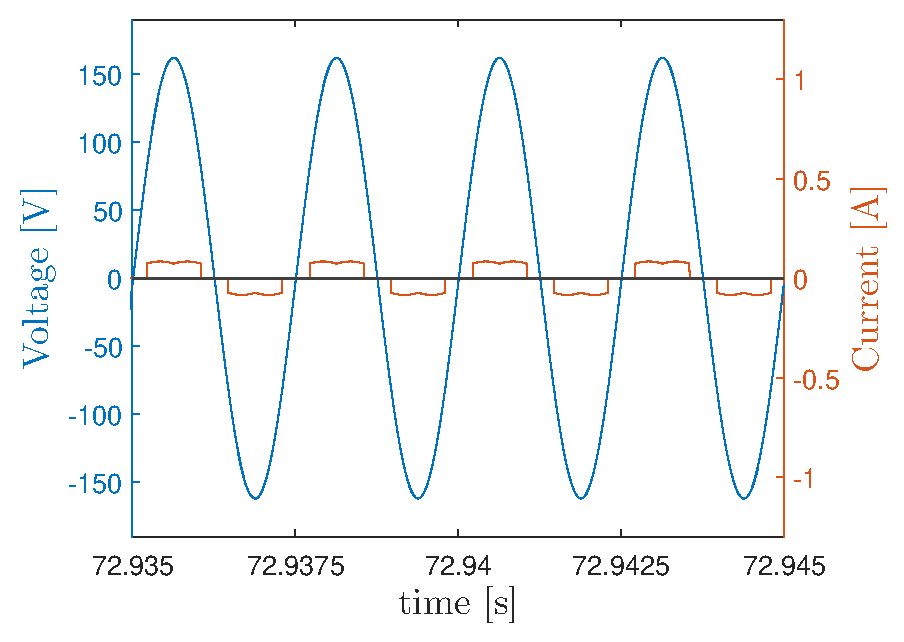
\includegraphics[width=0.27\textheight]{Figures/artigo_unfilt_1.eps}
	\caption{Voltage and current waveforms for the system without load and filter}
	\label{fig:artigo_unfilt_1.eps}
\end{figure}

\begin{figure}[!h] %
	\centering
	\includegraphics[width=0.27\textheight]{Figures/artigo_unfilt_2.eps}
	\caption{Voltage spectrum for the system without load and filter}
	\label{fig:artigo_unfilt_2.eps}
\end{figure}

\begin{figure}[!h] %
	\centering
	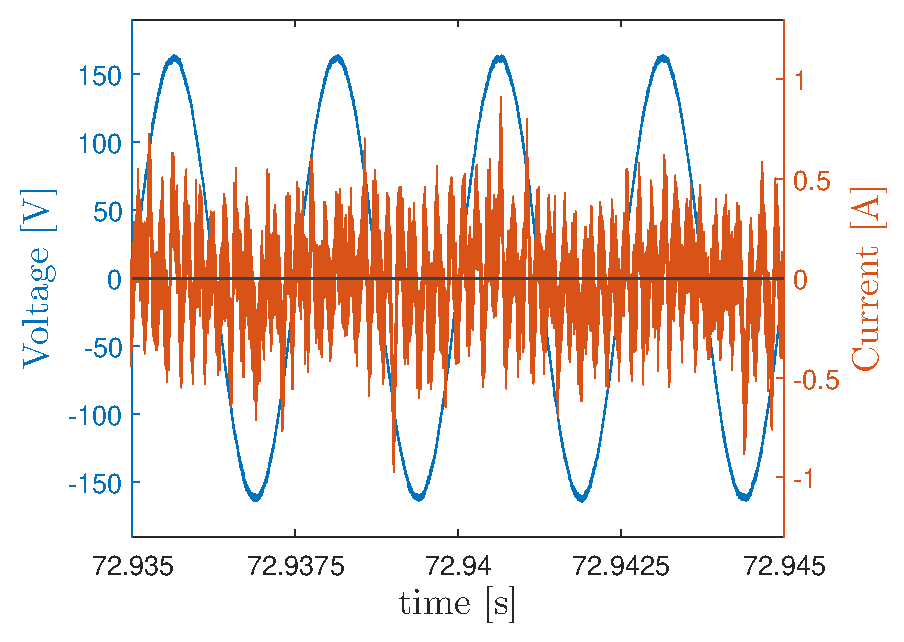
\includegraphics[width=0.27\textheight]{Figures/artigo_filt_1.eps}
	\caption{Voltage and current waveforms for the system without load and with filter}
	\label{fig:artigo_filt_1.eps}
\end{figure}

\begin{figure}[!h] %
	\centering
	\includegraphics[width=0.27\textheight]{Figures/artigo_filt_2.eps}
	\caption{Voltage spectrum for the system without load and with filter}
	\label{fig:artigo_filt_2.eps}
\end{figure}

\begin{figure}[!h] %
	\centering
	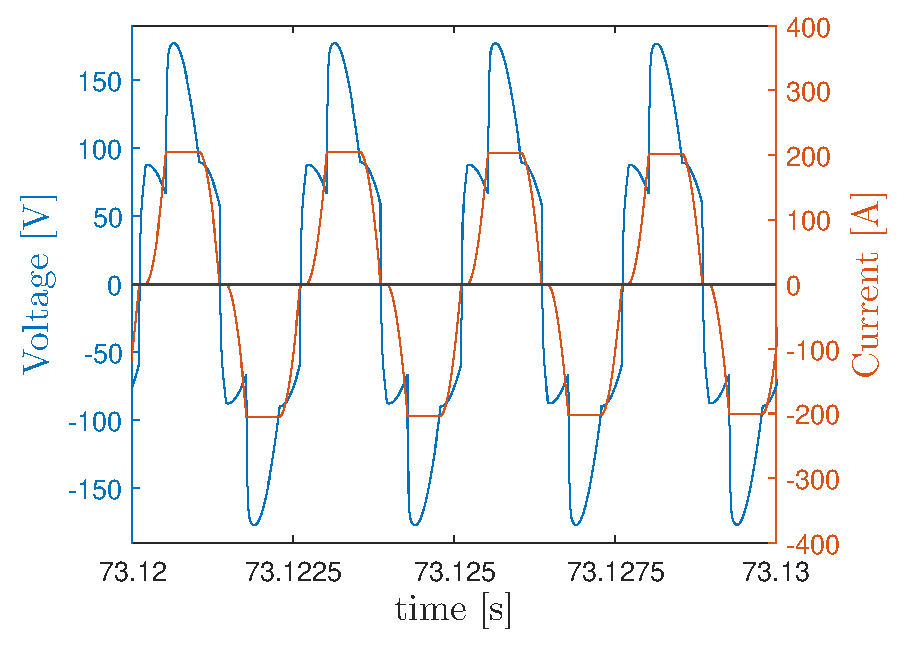
\includegraphics[width=0.27\textheight]{Figures/artigo_unfilt_3.eps}
	\caption{Voltage and current waveforms for the system with load and without filter}
	\label{fig:artigo_unfilt_3.eps}
\end{figure}

\begin{figure}[!h] %
	\centering
	\includegraphics[width=0.27\textheight]{Figures/artigo_unfilt_4.eps}
	\caption{Voltage spectrum for the system with load and without filter}
	\label{fig:artigo_unfilt_4.eps}
\end{figure}

\begin{figure}[!h] %
	\centering
	\includegraphics[width=0.27\textheight]{Figures/artigo_filt_3.eps}
	\caption{Voltage and current waveforms for the system with load and filter}
	\label{fig:artigo_filt_3.eps}
\end{figure}

\begin{figure}[!h] %
	\centering
	\includegraphics[width=0.27\textheight]{Figures/artigo_filt_4.eps}
	\caption{Voltage spectrum for the system with load and filter}
	\label{fig:artigo_filt_4.eps}
\end{figure}
